\subsection{Закон великих чисел (ЗВЧ).}

Маємо $\xi_1, \xi_2, ...$, тоді:
$$
\underbrace{\frac{\xi_1 + \xi_2 + ... + \xi_n}{n}}_{\text{вибіркове середнє}} \xrightarrow[n \to \i]{} \mathbb{E}\xi
$$
\begin{boxteo}(ЗВЧ для незалежних, однаково розподілених величин)\\
  $\xi_1, \xi_2, ..., \xi_n$ - незалежні, однаково розподілені випадкові величини.\\
  Нехай $\exists\mathbb{E}\xi_i = a$.
  \textbf{Тоді}:
  $$
  \frac{\xi_1 + ... + \xi_n}{n} \xrightarrow[n \to \i]{\mathbb{P}} a
\qquad
  \left( \mathbb{P} \left\lbrace \frac{\xi_1 + ... + \xi_n}{n}  > \varepsilon  \right\rbrace \xrightarrow[n \to \i]{} 0 \right)
  $$
\end{boxteo}
\begin{proof} ( за додаткової умови існування дисперсії $\exists\mathbb{D}\xi_i$, що , але з послабленим припущенням про некорельованість замість незалежності.)
$$
\overline{\xi} = \frac{\xi_1 + ... + \xi_n}{n} : \begin{gathered}
 \mathbb{E} \overline{\xi}_n= \mathbb{E}  \frac{\xi_1 + ... + \xi_n}{n}  = \frac{ \mathbb{E}\xi_1 + ... + \mathbb{E}\xi_n}{n}  = \frac{na}{a} = a \\
 \mathbb{D} \overline{\xi}_n = \mathbb{D} \frac{\xi_1 + ... + \xi_n}{n} = \frac{\mathbb{D}\xi_1 + ... + \mathbb{D}\xi_n}{n^2} =  \frac{n \mathbb{D} \xi}{ n^2} = \frac{\mathbb{D} \xi}{n}
\end{gathered}
$$
$$
\begin{dcases}
 \mathbb{E} \overline{\xi}_n = a \xrightarrow[n\to \i]{} a \\
 \mathbb{D} \overline{\xi}_n = \frac{\mathbb{D} \xi}{n} \xrightarrow[n\to \i]{} 0
 \end{dcases} \Longrightarrow \overline{\xi}_n \xrightarrow[n\to \i]{\mathbb{L}_2} a \Longrightarrow \overline{\xi}_n \xrightarrow[n\to \i]{\mathbb{P} } a
$$
\end{proof}
\begin{proof} (без припущення про існування $\mathbb{D} \xi$)\\
Введемо характеристичну функцію $ \char (t) = \mathbb{E} e^{it \xi}$. Тоді:
$$
    \chi_{\frac{\xi_1 + ... + \xi_n}{n}}(t) =  \mathbb{E} e ^{ \frac{it}{n} (\xi_1 + ... + \xi_n)  } = \chi_{\xi_1 + ... + \xi_n} \left( \frac{t}{n}  \right) = \underbrace{\char \left( \frac{t}{n}  \right)\cdot ... \cdot \char \left( \frac{t}{n}  \right)}_{n} = \char^n \left( \frac{t}{n}  \right)
$$
Розпишемо в ряд Тейлора:
$$
\char(h)  = \char(0) + \frac{\char'(0)}{1!} h + o(h) \quad h \to 0
$$
$$
\char(h)  =  \left| \frac{\char'(0)}{i}  = \mathbb{E}\xi \right|= 1 + ia\cdot h + o(h) \quad h \to 0
$$
$$
\char \left( \frac{t}{n} \right)   =  1 + \frac{iat}{n}  + o( \frac{1}{n} ) \quad n \to \i
$$
Отримали:
$$
\chi_{\overline{\xi}_n} (t) = \char^n \left( \frac{t}{n}  \right) = \left[ 1 + \frac{iat}{n}  + o  \left( \frac{1}{n} \right)\right]^n  \quad n \to \i
$$
$$
\ln{ \chi_{\overline{\xi}_n} (t) } = n \ln \left[ 1 + \frac{iat}{n}  + o  \left( \frac{1}{n} \right) \right] \sim n \left[ \frac{iat}{n} + o \left( \frac{1}{n}  \right)  \right] = iat + o(1) \xrightarrow[n\to \i]{} a
$$
$$
\chi_{\overline{\xi}_n} (t) \xrightarrow[ n \to \infty]{} e^{iat} = \mathbb{E} e^{iat}= \char (t) \quad \fbox{$\xRightarrow{\text{т. Леві}}$}
$$
$$
\fbox{$\Longrightarrow$} \overline{\xi}_n = \frac{\xi_1 + ... + \xi_n}{n} \xrightarrow[n\to\i]{d}a \Rightarrow \fbox{$\dfrac{\xi_1 + ... + \xi_n}{n} \xrightarrow[n\to\i]{\mathbb{P}} a$}
$$
\end{proof}
\begin{boxteo}(посилений ЗВЧ А.М.Колмогорова.)\\
$\xi_1, \xi_2, ..., \xi_n$ - незалежні, однаково розподілені випадкові величини.
$$
\text{Нехай } \exists\mathbb{E}\xi_i = a.\
\textbf{Тоді:}\  \frac{\xi_1 + ... + \xi_n}{n} \xrightarrow[n \to \i]{\textbf{м.н.}} a
$$
Без доведення.\ \ $\blacksquare$
\end{boxteo}
\newpage
\subsection{ЗВЧ для різнорозподілених випадкових величин.}
\subsubsection{Формулювання.}
\vfill
\begin{boxteo}
$\xi_1, \xi_2, ..., \xi_n$ - незалежні випадкові величини.
Нехай $\begin{gathered}
 \exists\mathbb{E}\xi_i = a_i\\
 \exists \mathbb{D} \xi_i = \sigma^2_i
\end{gathered}$. \\ Додатково накладемо умову рівномірної обмеженості:  $\exists C > 0:  \sigma^2_i < C $.
$$
 \textbf{Тоді:} \ \frac{ \xi_1 + ... + \xi_n}{n} - \frac{a_1 + ... + a_n}{n} = \frac{(\xi_1 - a_1) + ... + (\xi_n - a_n)}{n}   \xrightarrow[n\to \i]{\mathbb{P}, \mathbb{L}_2} 0
$$
\end{boxteo}
\vfill
\begin{proof}
 $$
 \begin{dcases}
   \mathbb{E} \left( \frac{(\xi_1 - a_1) + ... + (\xi_n - a_n)}{n}  \right)= \frac{\overbrace{\mathbb{E}(\xi_1 - a_1)}^{=0} + ... +\overbrace{\mathbb{E}(\xi_n - a_n)}^{=0}}{n} =  0  & \xrightarrow[n\to\i]{} 0\\
   \mathbb{D} \left(  \frac{(\xi_1 - a_1) + ... + (\xi_n - a_n)}{n} \right) =   \frac{\mathbb{D}(\xi_1 - a_1) + ... + \mathbb{D}(\xi_n - a_n)}{n^2} = \\
   = \frac{\mathbb{D} \xi_1 + ... + \mathbb{D}\xi_n}{n} - \frac{a_1 + ... + a_n}{n^2} = \frac{\sigma_1 ^2 + ... + \sigma_n^2}{n^2} \leq \frac{C\cdot n}{n^2} = \frac{C}{n} &\xrightarrow[n\to\i]{} 0
 \end{dcases}
 $$
 З цього слідує: $ \frac{(\xi_1 - a_1) + ... + (\xi_n - a_n)}{n} \xrightarrow[n\to\i]{\mathbb{L}_2, \mathbb{P}}
 0 $
\end{proof}
\vfill
\subsubsection{ЗВЧ для схеми Бернуллі.}
Успіх: $p$. Невдача: $q = 1 - p$. \\
Введемо величину $\xi_i = \index{} \left\lbrace \text{на i-тому випробуванні відбувся успіх} \right\rbrace$
$$
\begin{gathered}
  \begin{gathered}
   \xi_i \\
   \mathbb{P}
  \end{gathered}
  \
  \begin{gathered}
   0\\
   q
  \end{gathered}
  \
  \begin{gathered}
   1 \\
   p
  \end{gathered} \quad \mathbb{E} \xi_i = p
\end{gathered}
$$
За ЗВЧ Колмогорова:
$$
\frac{\xi_1 + ... + \xi_n}{n} \xrightarrow[n \to \i]{\mathbb{L}_2, \mathbb{P}, \text{м.н}}  \mathbb{E} \xi_i = p
$$
$\frac{\xi_1 + ... + \xi_n}{n} $ - відносна частота успіхів $ = \nu_n \Longrightarrow $ \fbox{ $\nu_n \xrightarrow[n \to \i]{\mathbb{L}_2, \text{м.н}} p $}
\vfill
\newpage
\subsubsection{Методи Монте-Карло.}
\textbf{Приклад.} Методи Монте-Карло дозволяють чисельно розв'язувати нестохастичні (детерміновані) задачі задопомогою стохастичних методів.\\
Шукаємо приблизне значення
$ \displaystyle \int\limits_{b}^{a}{f(x)dx }$ при  $ M \geq  f(x) \geq 0 $ -  обмежена на $[a,b]$ .\\
\begin{center}
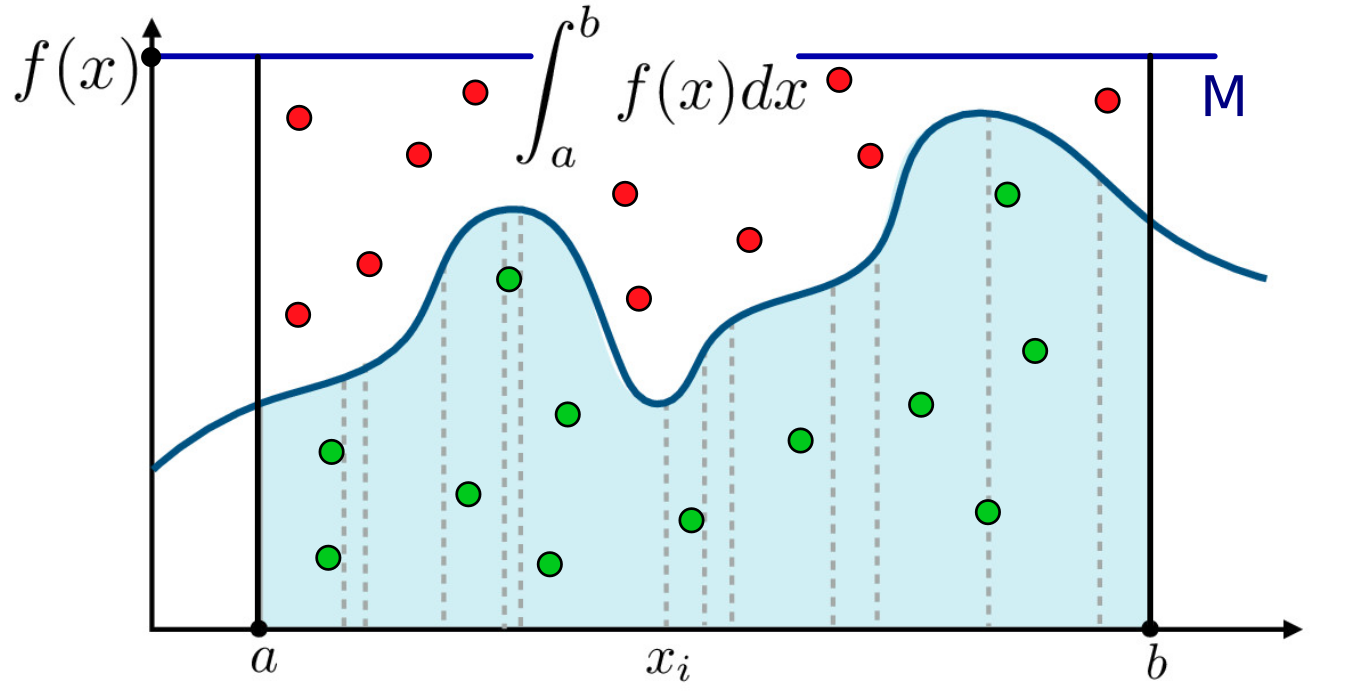
\includegraphics[scale=0.33]{assets/lectures_part_4-fdb5d503.png}
Вибираємо незалежні: $\xi_n \sim U(a,b)$.
\end{center}
$f(\xi_1), ... f(\xi_n) $ - незалежні, однаково розподілені з математичним сподіванням:
$$
\mathbb{E} f(\xi_i) =  \int\limits_{b}^{ a}{ f(x) \cdot \frac{1}{b-a}dx } = \frac{1}{b-a}  \int\limits_{b}^{a}{f(x)dx}
$$
Застосуємо закон великих чисел:
$$
\frac{f(\xi_1) + ... + f(\xi_n)}{n} \xrightarrow[n \to \i]{\text{м.н.}}  \mathbb{E} f(\xi)
$$
Якщо взяти $ n >> 1$:
$$
\frac{f(\xi_1) + ... + f(\xi_n)}{n} \approx \frac{1}{b-a}  \int\limits_{b}^{a}{f(x)dx}
$$
Інакше:
$$  \int\limits_{b}^{a}{f(x)dx} \approx \left( b-a \right)\cdot \frac{f(\xi_1) + ... + f(\xi_n)}{n}$$
\begin{example}(Другий спосіб) Розглядаємо прямокутник $\Pi = (a,b) \times M$.\\
Випадкові вектори $\begin{bmatrix}
 \xi_1 \\
 \eta_1
\end{bmatrix}, \cdots , \begin{bmatrix}
 \xi_n\\
 \eta_n
\end{bmatrix} $ - точки всередині прямокутника $ \Pi$.\\
Схема Бернуллі: $n$ випробувань. Успіх: потрапляння точки під графік $f(x)$.
$$
p = \mathbb{P} \left\lbrace \text{успіх} \right\rbrace = \frac{S_{\text{під графіком}}}{S_{\Pi}} =
\frac{ \int\limits_{b}^{a}{f(x)dx}}{M(b-a)}
$$
Частота влучання під графік: $\nu_n \xrightarrow[n \to \i]{\text{м.н}} p = \frac{ \int\limits_{b}^{a}{f(x)dx}}{M(b-a)}  $.\\
Якщо $ n >> 1$, то $ \int\limits_{b}^{a}{f(x)dx} \approx M(b-a)\nu_n = M(b-a)\cdot \frac{\text{к-сть точок під графіком}}{n} $.

\end{example}

\vfill
\subsection{Центральна гранична теорема та її застосування.}
\subsubsection{Формулювання.}
\begin{boxteo}(Для незалежних, однаково розподілених величин).\\
$\xi_1, \xi_2, ..., \xi_n$ - незалежні, однаково розподілені випадкові величини.\\
Нехай $\exists\mathbb{E}\xi_i = m \ \ \exists \mathbb{D} \xi_i = \sigma^2$.
$$
\textbf{Тоді}: \
\frac{(\xi_1 - m) + ... + (\xi_n - m)}{\sigma\sqrt{n}}  \xrightarrow[n \to \i]{d} \gamma \sim N(0,1)$$
Неформально говорячи, класична ЦГТ стверджує, що сума з $n$ незалежних величин однаково розподілених має розподіл, близький до $N(nm, n \sigma^2)$.\\
Якою б не була форма розподілу генеральної сукупності, вибірковий розподіл наближається до нормального, а його дисперсія задається ЦГТ.
\begin{center}
 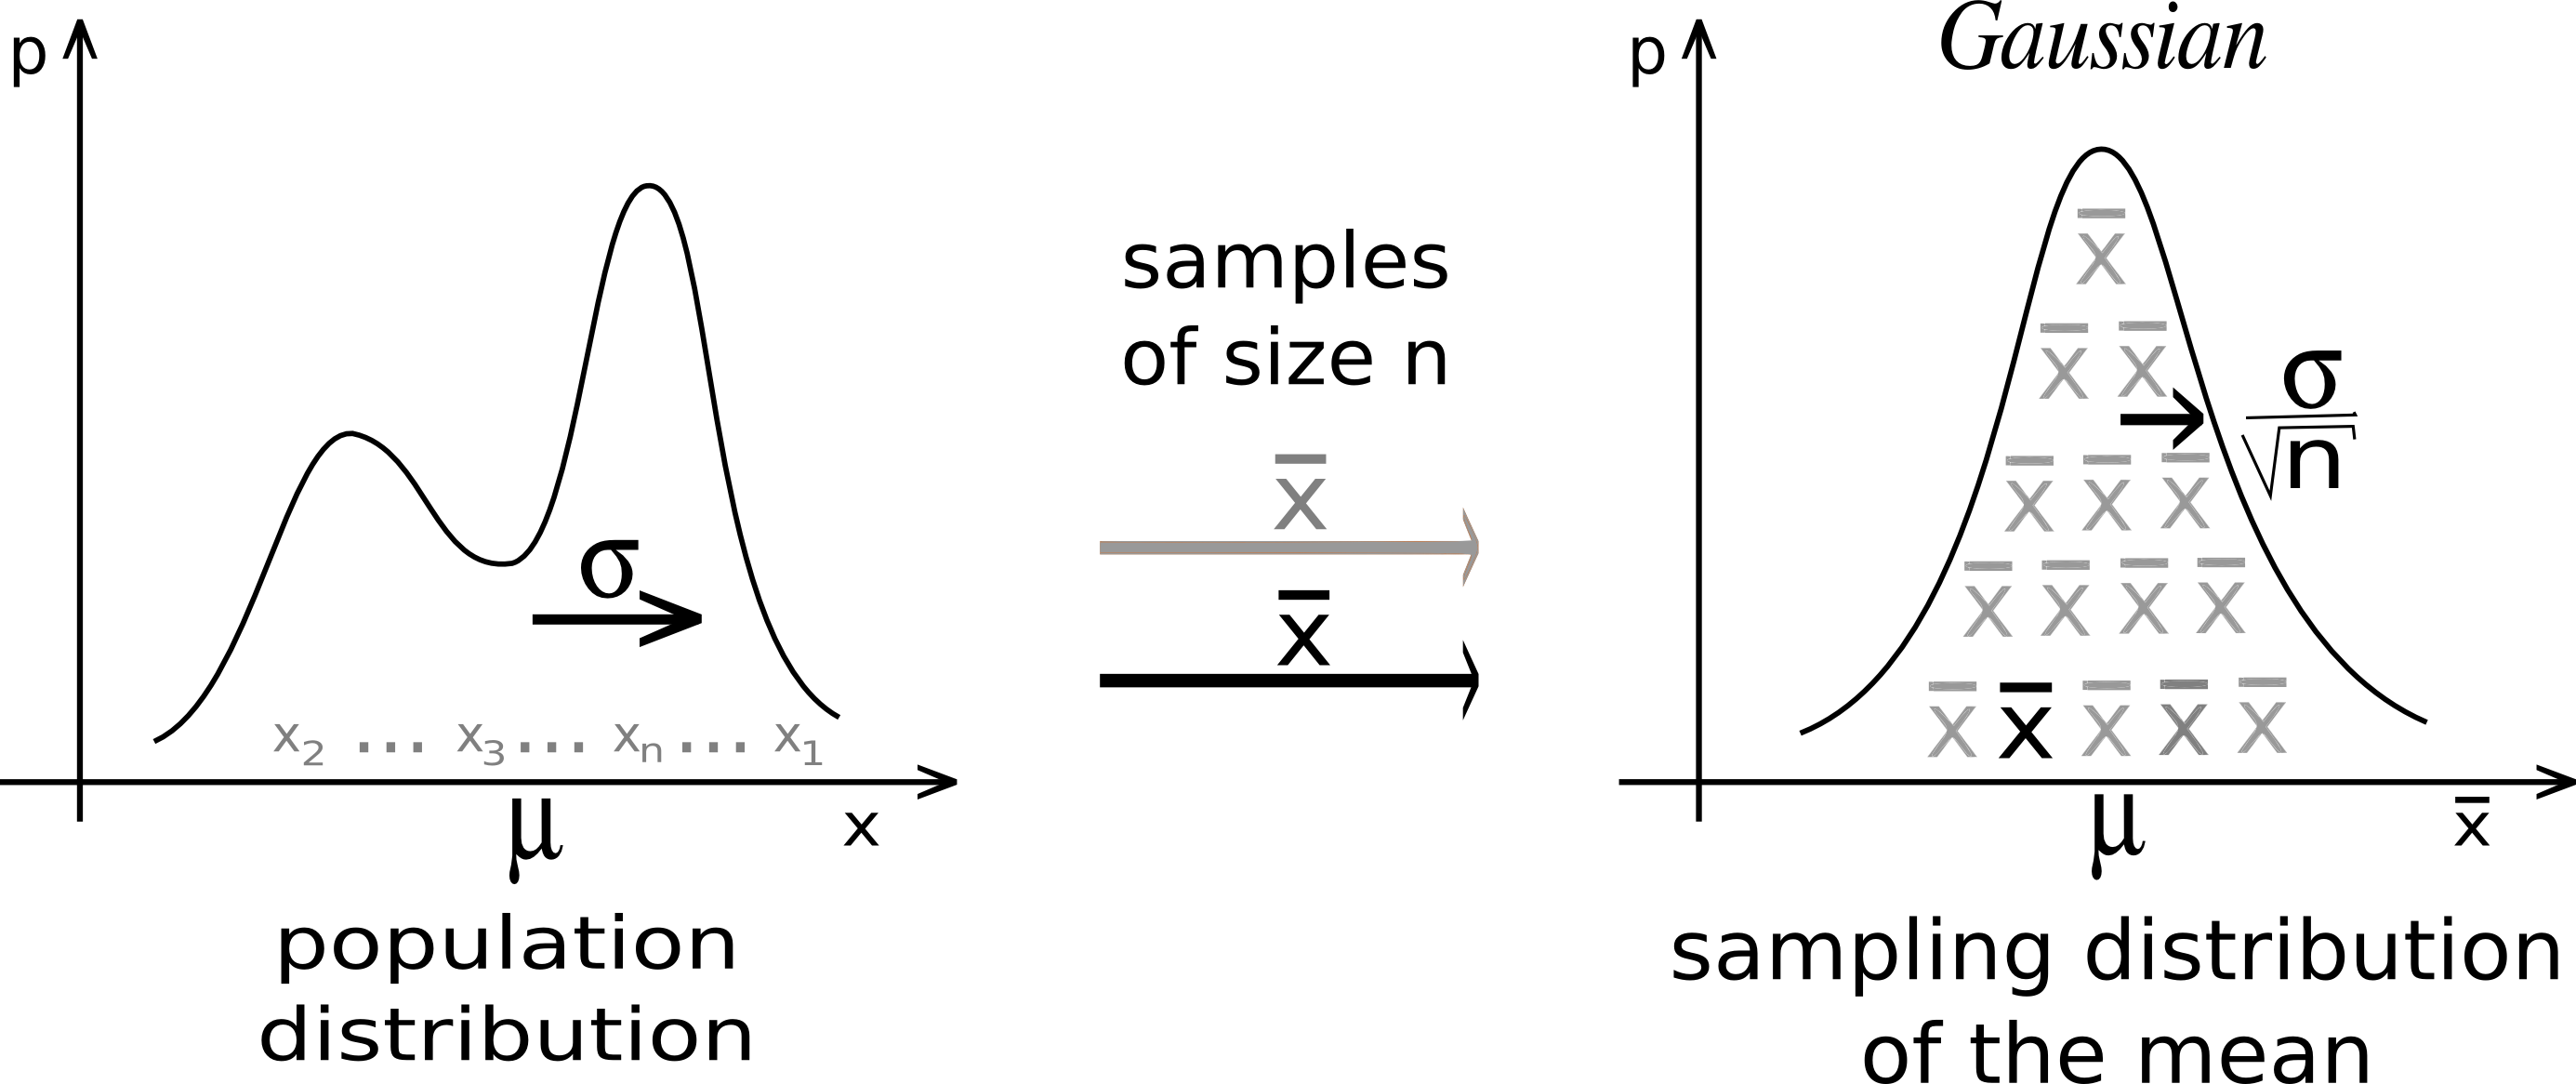
\includegraphics[scale=0.14]{assets/lectures_part_4-4d255f56.png}
\end{center}
\end{boxteo}
\newpage
\begin{proof}$ \xi_1, \xi_2, ..., \xi_n$ - незалежні, однаково розподілені випадкові величини.\\
Будемо позначати: $\xi_1 - m = \eta_1 \ \cdots \ \xi_n - m = \eta_n$. Тоді:
$$
\mathbb{E} \eta_i = \mathbb{E}(\xi_i - m) = \mathbb{E}\xi_i - m = m-m  = 0 \qquad \chi(t) = \chi_{\eta_i}(t)
$$
$$
\chi_{ \frac{\eta_1 + ... + \eta_n }{\sigma \sqrt{n}} } (t) = \mathbb{E} \exp \left\lbrace it \cdot  \frac{\eta_1 + ... + \eta_n }{\sigma \sqrt{n}}  \right\rbrace = \chi_{\eta_1 + ... + \eta_n} \left( \frac{t}{\sigma \sqrt{n}}  \right) = \chi^n \left( \frac{t}{\sigma \sqrt{n}}  \right)
$$
Хочемо знайти границю характеристичноъ функції на $n\to\i$. Позначимо:
$$
\lim\limits_{n\to  \infty}{ \chi_{\frac{(\xi_1 - m) + ... + (\xi_n - m)}{\sigma\sqrt{n}}}} (t) = L(t) =  \lim\limits_{n\to  \infty}{\chi^n \left( \frac{t}{\sigma \sqrt{n}}   \right)}
$$
$$
\ln L(t) = \lim\limits_{n\to  \infty}{n \ln \chi \left( \frac{t}{\sigma \sqrt{n}}   \right)} \circled{=}
 $$
 Розпишемо характеристичну функцію у ряд Тейлора:
 $$
 \chi (h) = \chi_{\eta}(h) = \chi(0) + \frac{\chi'(0)}{1!} h +  \frac{\chi''(0)}{2!} h^2 + o(h^2)= \qquad h \to 0
 $$
 $$
 =
\left|  \begin{gathered}
   \frac{\chi'(0)}{i} = \mathbb{E} \eta = 0\\
   \frac{\chi''(0)}{i^2} = -\mathbb{E} \eta^2 = -\mathbb{D} \eta =-\sigma ^2
 \end{gathered} \right| =  1 - \frac{\sigma ^2 }{2} h^2 + o(h^2) \qquad h \to 0
 $$
 $$
 \chi \left( \frac{t}{\sigma \sqrt{n}} \right) = 1 - \frac{\sigma ^2}{2} \cdot \frac{t^2}{n \sigma^2}  + o \left(  \frac{t}{\sigma \sqrt{n}}  \right)  = 1 - \frac{t^2}{2n} + o \left( \frac{1}{n} \right)   \qquad n \to +\i
 $$
 Підставивши у границю, отримаємо:
 $$
 \circled{=}  \lim\limits_{n\to  \infty}{n \cdot \ln \left( 1 - \frac{t^2}{2n} + o \left( \frac{1}{n} \right)  \right)} =  \lim\limits_{n\to  \infty}{n \left(  - \frac{t^2}{2n} + o \left( \frac{1}{n}  \right)  \right)}  = - \frac{t^2}{2}
 $$
 Отже, для початкової границі маємо:
 $$
  \lim\limits_{n\to  \infty}{ \chi_{\frac{(\xi_1 - m) + ... + (\xi_n - m)}{\sigma\sqrt{n}}}} (t) = L(t) =  e^{- \frac{t^2}{2} } = \chi_{N(0,1)}(t) \quad \forall t \in \mathbb{R} \quad \fbox{$\xRightarrow{\text{т. Леві}}$}
 $$
 $$
 \fbox{$\Longrightarrow$} \quad \frac{(\xi_1 - m) + ... + (\xi_n - m)}{\sigma\sqrt{n}} \xrightarrow[n\to\i]{d} \gamma \sim N(0,1)
 $$
\end{proof}
\begin{remark}
При великих $n$: $S_n = \xi_1 + ... + \xi_n \approx N(nm, n \sigma^2)$. Тоді:
$$
\mathbb{P} \left\lbrace a \leq  S_n \leq  \right\rbrace \approx \mathbb{P} \left\lbrace  a \leq  \gamma_n \leq b \right\rbrace = \Laplas \left( \frac{b - mn}{\sigma \sqrt{n}}  \right) - \Laplas \left( \frac{a - mn}{\sigma \sqrt{n}}  \right)
$$
\end{remark}
\newpage
\subsubsection{Використання ЦГТ у схемі Бернуллі.}
\begin{itemize}
    \item $p$ - імовірність успіху.
    \item $q = 1-p$ - імовірність невдачі.
    \item $\varepsilon_i = \index{}\left\lbrace \text{на і-тому випробуванні - успіх} \right\rbrace \in \left\lbrace 0,1 \right\rbrace$
    \item $
    \mathbb{E} \epsilon_i = 1 \cdot p + 0 \cdot q  = p
    $
    \item $\mathbb{E} \varepsilon_i^2 = 1^2\cdot p + 0^2 \cdot q = p$
    \item $\mathbb{D}\varepsilon _i = \mathbb{E} (\varepsilon _i)^2 - (\mathbb{E} \varepsilon _ i)^2$
\end{itemize}
$$
S_n =  \sum\limits_{i = 1}^{ n}{ \varepsilon_i} \quad \Longrightarrow \quad n>>1 : \text{ ЦГТ } S_n \approx N(nm, n \sigma ^2) = N(np, npq)
$$
\begin{center}
 \textbf{Інтегральна формула Муавра-Лапласа}
\end{center}
$$
\mathbb{P} \left\lbrace a \leq  S_n  \leq b \right\rbrace \approx \Laplas \left( \frac{b - np}{ \sqrt{npq}}  \right) - \Laplas \left( \frac{a - np}{\sqrt{npq}}  \right) \approx \Laplas \left( \frac{b + \frac{1}{2}  - np}{ \sqrt{npq}}  \right) - \Laplas \left( \frac{a - \frac{1}{2}  - np}{\sqrt{npq}}  \right)
$$
Можемо використовувати, якщо: $\begin{dcases}
 n\geq 50\\
 npq \geq 10
\end{dcases}$. \  $\circledast$\\
Якщо $n$ мале, користуємося точною формулою:
$$
\mathbb{P} \left\lbrace a \leq S_n \leq b \right\rbrace =  \sum\limits_{k = a}^{ b}{ \mathbb{P} \left\lbrace S_n =k \right\rbrace} =  \sum\limits_{k = a}^{ b}{ C_n^k p^k q^{n-k}}
$$
Якщо $p$ близьке до 1 або до 0, застосовуємо граничну теорему Пуассона.
\subsubsection{Локальна формула Муавра-Лапласа.}
Якщо виконуються умови $\circledast$:


$$
\mathbb{P} \left\lbrace S_n = k \right\rbrace = \mathbb{P} \left\lbrace k \leq S_n \leq k \right\rbrace \approx\Laplas \left( \frac{k + \frac{1}{2}  - np}{ \sqrt{npq}}  \right) - \Laplas \left( \frac{k - \frac{1}{2}  - np}{\sqrt{npq}}  \right) \circled{=}
$$
За теоремою Лагранжа:
$$
f(b) - f(a) = f'(x) (b-a) \qquad b-a =   \frac{k + \frac{1}{2}  - np}{ \sqrt{npq}}  -  \frac{k - \frac{1}{2}  - np}{\sqrt{npq}}  = \frac{1}{ \sqrt{npq}}
$$
$$
\circled{=} \  \frac{1}{ \sqrt{npq}} \cdot \frac{1}{\sqrt{2 \pi}} e^{- \frac{x^2}{2} } \approx \frac{1}{\sqrt{2\pi n p q}} \cdot e^{- \frac{x^2}{2} } \bigg|_{x = \frac{k- np}{\sqrt{npq}} }
$$
\begin{center}
 \textbf{Локальна формула Муавра-Лапласа}
\end{center}
$$
\mathbb{P} \left\lbrace  S_n = k \right\rbrace \approx \frac{1}{\sqrt{2 \pi npq}} \exp \left\lbrace - \frac{(k-np)^2}{2npq}  \right\rbrace
$$
\subsubsection{Теорема Пуассона}
\begin{boxteo} [Пуассона]
Нехай є послідовність схем Бернуллі:\\
\quad 1. Одне випробування з $p_1$ - імовірність успіху.\\
\quad 2. Два випробування з $p_2$ - імовірність успіху.\\
$\qquad \cdots \qquad \cdots \qquad \cdots$\\
\quad n. n випробувань з $p_n$ - імовірність успіху.\\
Нехай є величина $\nu_n$ - кількість успіхів в n-тій схемі Бернуллі.\\
\textbf{Якщо} $b\cdot p_n \xrightarrow[n\to\infty]{} \lambda > 0$,\\
\textbf{тоді:} $\nu_n \xrightarrow[n\to\infty]{d} \theta \sim Pois(\lambda) \ : \  \mathbb{P} \left\lbrace \theta = k \right\rbrace = \dfrac{e^{-\lambda} \lambda^k}{k!} $.
\end{boxteo}
\begin{remark} Якщо виконується зазначена збіжність:
$$
\mathbb{P} \left\lbrace \nu_n = k \right\rbrace \xrightarrow[n\to\infty]{} \underbrace{\mathbb{P} \left\lbrace \theta = k \right\rbrace}_{\frac{e^{-\lambda} \lambda^k}{k!} } \quad \forall k \in \overline{1,n}
\ \ \Longrightarrow \ \
\forall x \notin \overline{0,1}  \quad F_{\nu_n} \xrightarrow[n\to\infty]{} F_{Pois(\lambda)} (x)
$$
$$
\mathbb{P} \left\lbrace \nu_n = k \right\rbrace = \mathbb{P} \left\lbrace \nu_n \in \left[ k- \frac{1}{2}, k+ \frac{1}{2} \right]   \right\rbrace = F_{\nu_n} \left( k + \frac{1}{2}  \right) - F_{\nu_n} \left( k - \frac{1}{2}  \right) \xrightarrow[n\to\infty]{}
$$
$$
\longrightarrow F_{\theta} \left( k + \frac{1}{2}  \right) - F_{\theta} \left( k - \frac{1}{2}  \right) = \mathbb{P} \left\lbrace \theta \in \left[ k- \frac{1}{2}, k+ \frac{1}{2}  \right] \right\rbrace = \mathbb{P} \left\lbrace \theta = k \right\rbrace
$$
\end{remark}
\begin{proof} Покажемо збіжність $\nu_n \xrightarrow[n\to\infty]{d} \theta$.
 $$
 \begin{gathered}
    \nu_n \sim Bin(n,p_n) \\ \theta \sim Pois(\lambda) \\ np_n \xrightarrow[n\to\infty]{} \lambda
 \end{gathered} \quad \Rightarrow \quad \begin{gathered}
    \underbrace{\left( p_n e^{it} + q_n \right)^n}_{= \left( p_n e^{it} + 1-p_n \right)^n} = \chi_{\nu_n} \xrightarrow[n\to\infty]{?}\chi_{\theta}(t) = e^{\lambda \left( e^{it} -1 \right)}\\
    \text{Позначимо: } \  L(t) =  \lim\limits_{n\to  \infty}{\left( p_n e^{it} + 1-p_n \right)^n}
 \end{gathered}
 $$
 $$
 \ln L(t) =  \lim\limits_{n\to  \infty}{\ln \left( p_n e^{it} + 1-p_n \right)^n} =  \lim\limits_{n\to  \infty}{ n \cdot \ln \left(1 + \underbrace{p_n (e^{it}-1) }_{\to 0} \right)^n} =  \lambda (e^{it} - 1)
 $$
 $$
 L(t) = e^{\lambda(e^{it} -1 )} = \chi_{Pois(\lambda)}(t) \quad \forall t \in \mathbb{R} \quad \text{Q.E.D.}
 $$
\end{proof}
\subsubsection{Наближена формула Пуассона у схемі Бернуллі.}
Якшо у серії із $n$ випробувань Бернуллі: $n\geq 50 \ \  npq \leq 10$.
$$
\fbox{$p \approx 0$} \qquad \mathbb{P} \left\lbrace \nu_k = k \right\rbrace \approx \frac{e^{-\lambda}\lambda^k}{k!} \quad k \in \overline{1,n} \quad \underline{\lambda =  np}
$$
